\documentclass[12pt,twoside,a4paper]{report}
%\usepackage[utf8x]{inputenc}
\usepackage{natbib}
%\usepackage{a4wide}
\usepackage{graphicx}
\usepackage{amsmath}
\usepackage{color}
\usepackage[usenames,dvipsnames]{xcolor}
\usepackage[cm]{fullpage}
\usepackage{hyperref}
%\usepackage{coffee4}
\frenchspacing
%opening

\begin{document}

\begin{titlepage}

\centering
 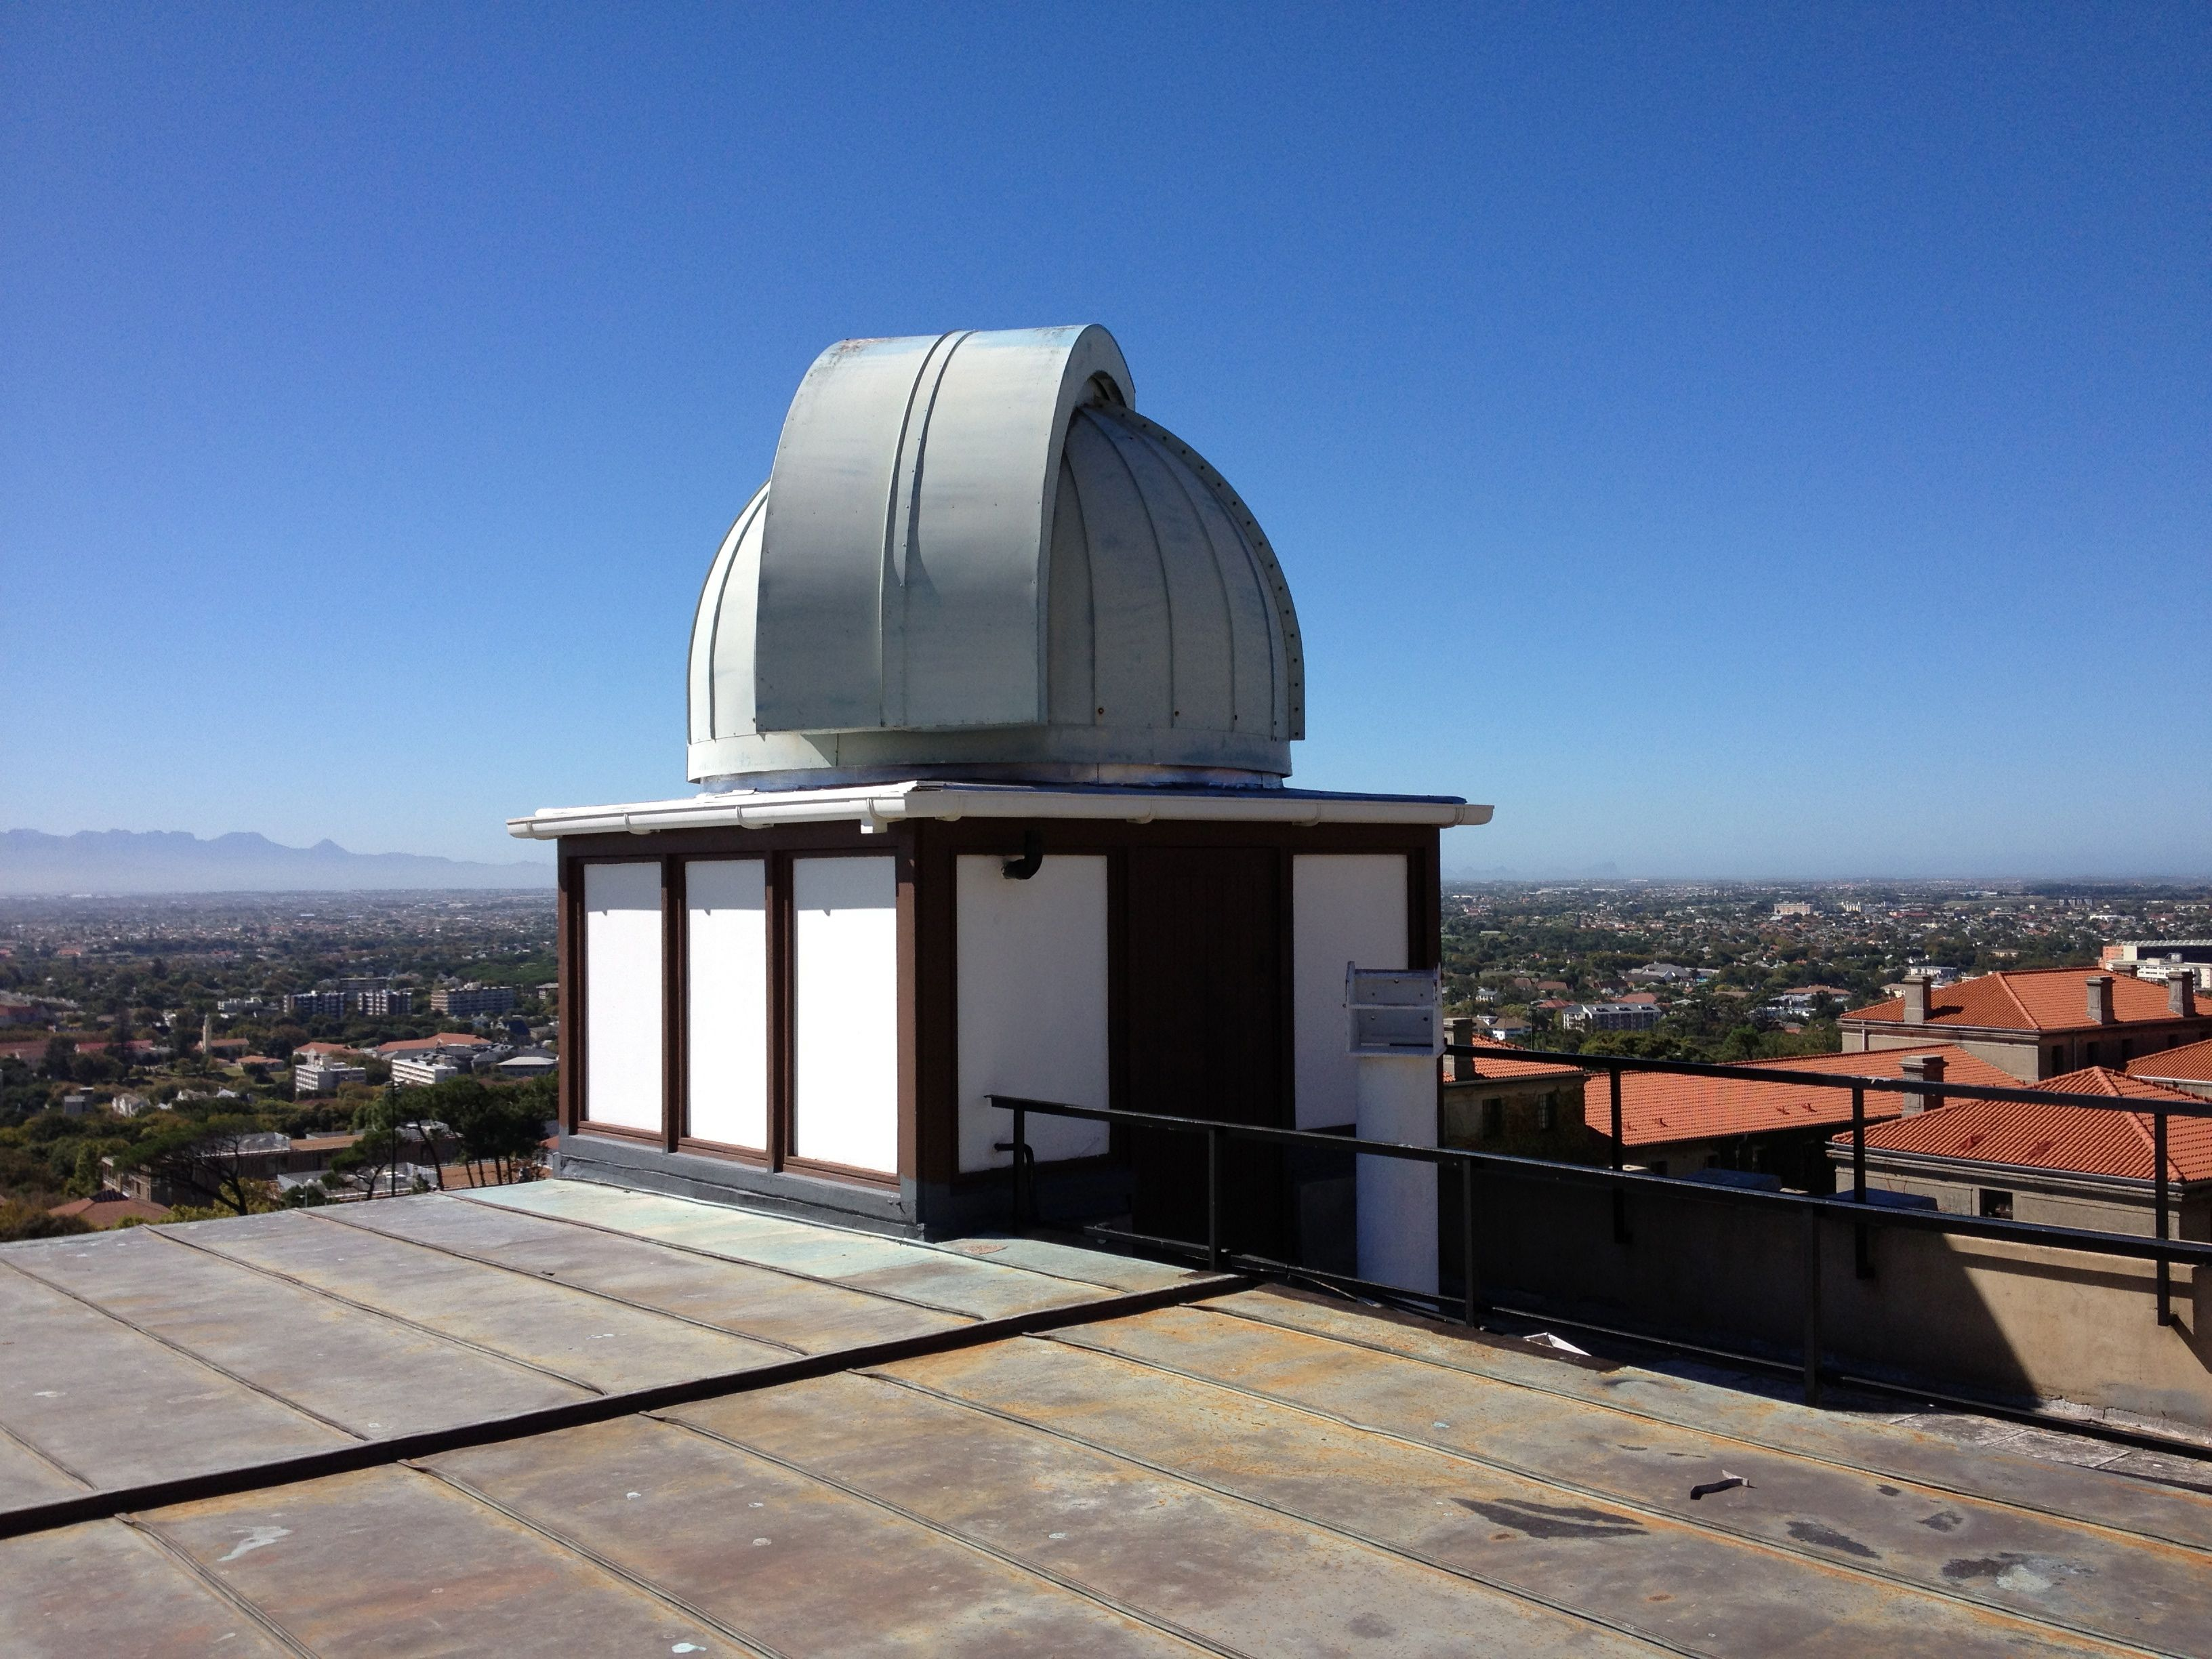
\includegraphics[width=15cm]{documentation_images/Dome14in.jpg}

\vspace{2cm}
{\Huge User's Guide to the UCT 14 Inch telescope}

\vspace{1cm}

{\small
Thuso Simon \\
thuso@ast.uct.ac.za \\
Version $0.1$}

\end{titlepage}

\tableofcontents


\chapter{The UCT Teaching Observatory}

This document is a user's guide to use the 14-inch Celestron telescope housed at the UCT Teaching Observatory
on campus. This is a modern telescope that is used for teaching and simple astronomy projects. This guide will 
help you to understand and use the telescope and highlights the operational procedures. Read this document
carefully to ensure the safe use of the telescope.\\

Chapter 2 of this document describes all basic observing procedures, including the start-up and shut-down sequence,
the telescope control via dedicated software (\emph{The SkyX}), the CCD camera control via its dedicated
software (\emph{Maxim DL}), target acquisition and auto-guiding.\\

Chapter 3 outlines a number of advanced observing procedures, including remote observing and details of 
instrument changes.\\

Chapter 4 highlights general guidelines for photometry.\\

\begin{figure}[h]
 \centering
    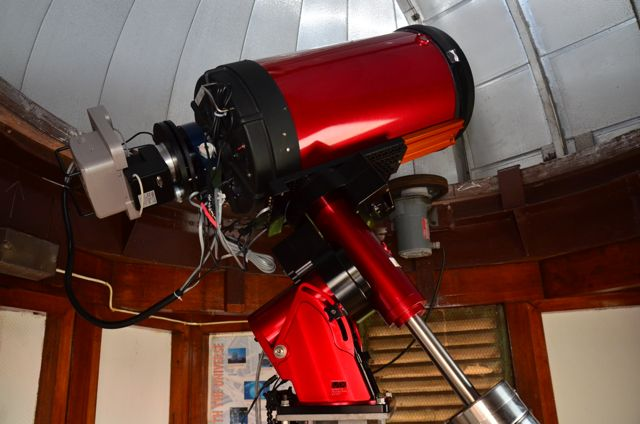
\includegraphics[width=0.75\textwidth]{documentation_images/telescope.jpg}
    \caption{\label{fig:telescope} The 14-inch Celestron at the Teaching Observatory.}
\end{figure}

\vfill \eject

\chapter{Basic Observing Procedures}

\section{Start up procedures}

This chapter describes the basic observing procedures on the 14-inch UCT teaching telescope. 
Step-by-step instructions are given in this Section and
summarised in Section~\ref{checklists}.

\subsection{Connecting the laptop}

The first step is the connect the observatory laptop to the power socket and internet cable. Make
sure that the dome control USB and the telescope control USB cables are connected to the laptop.
Turn on all the power switches in the dome (on the east and South wall of the dome) and start the
(windows) laptop.

\begin{figure}[h]
 \centering
    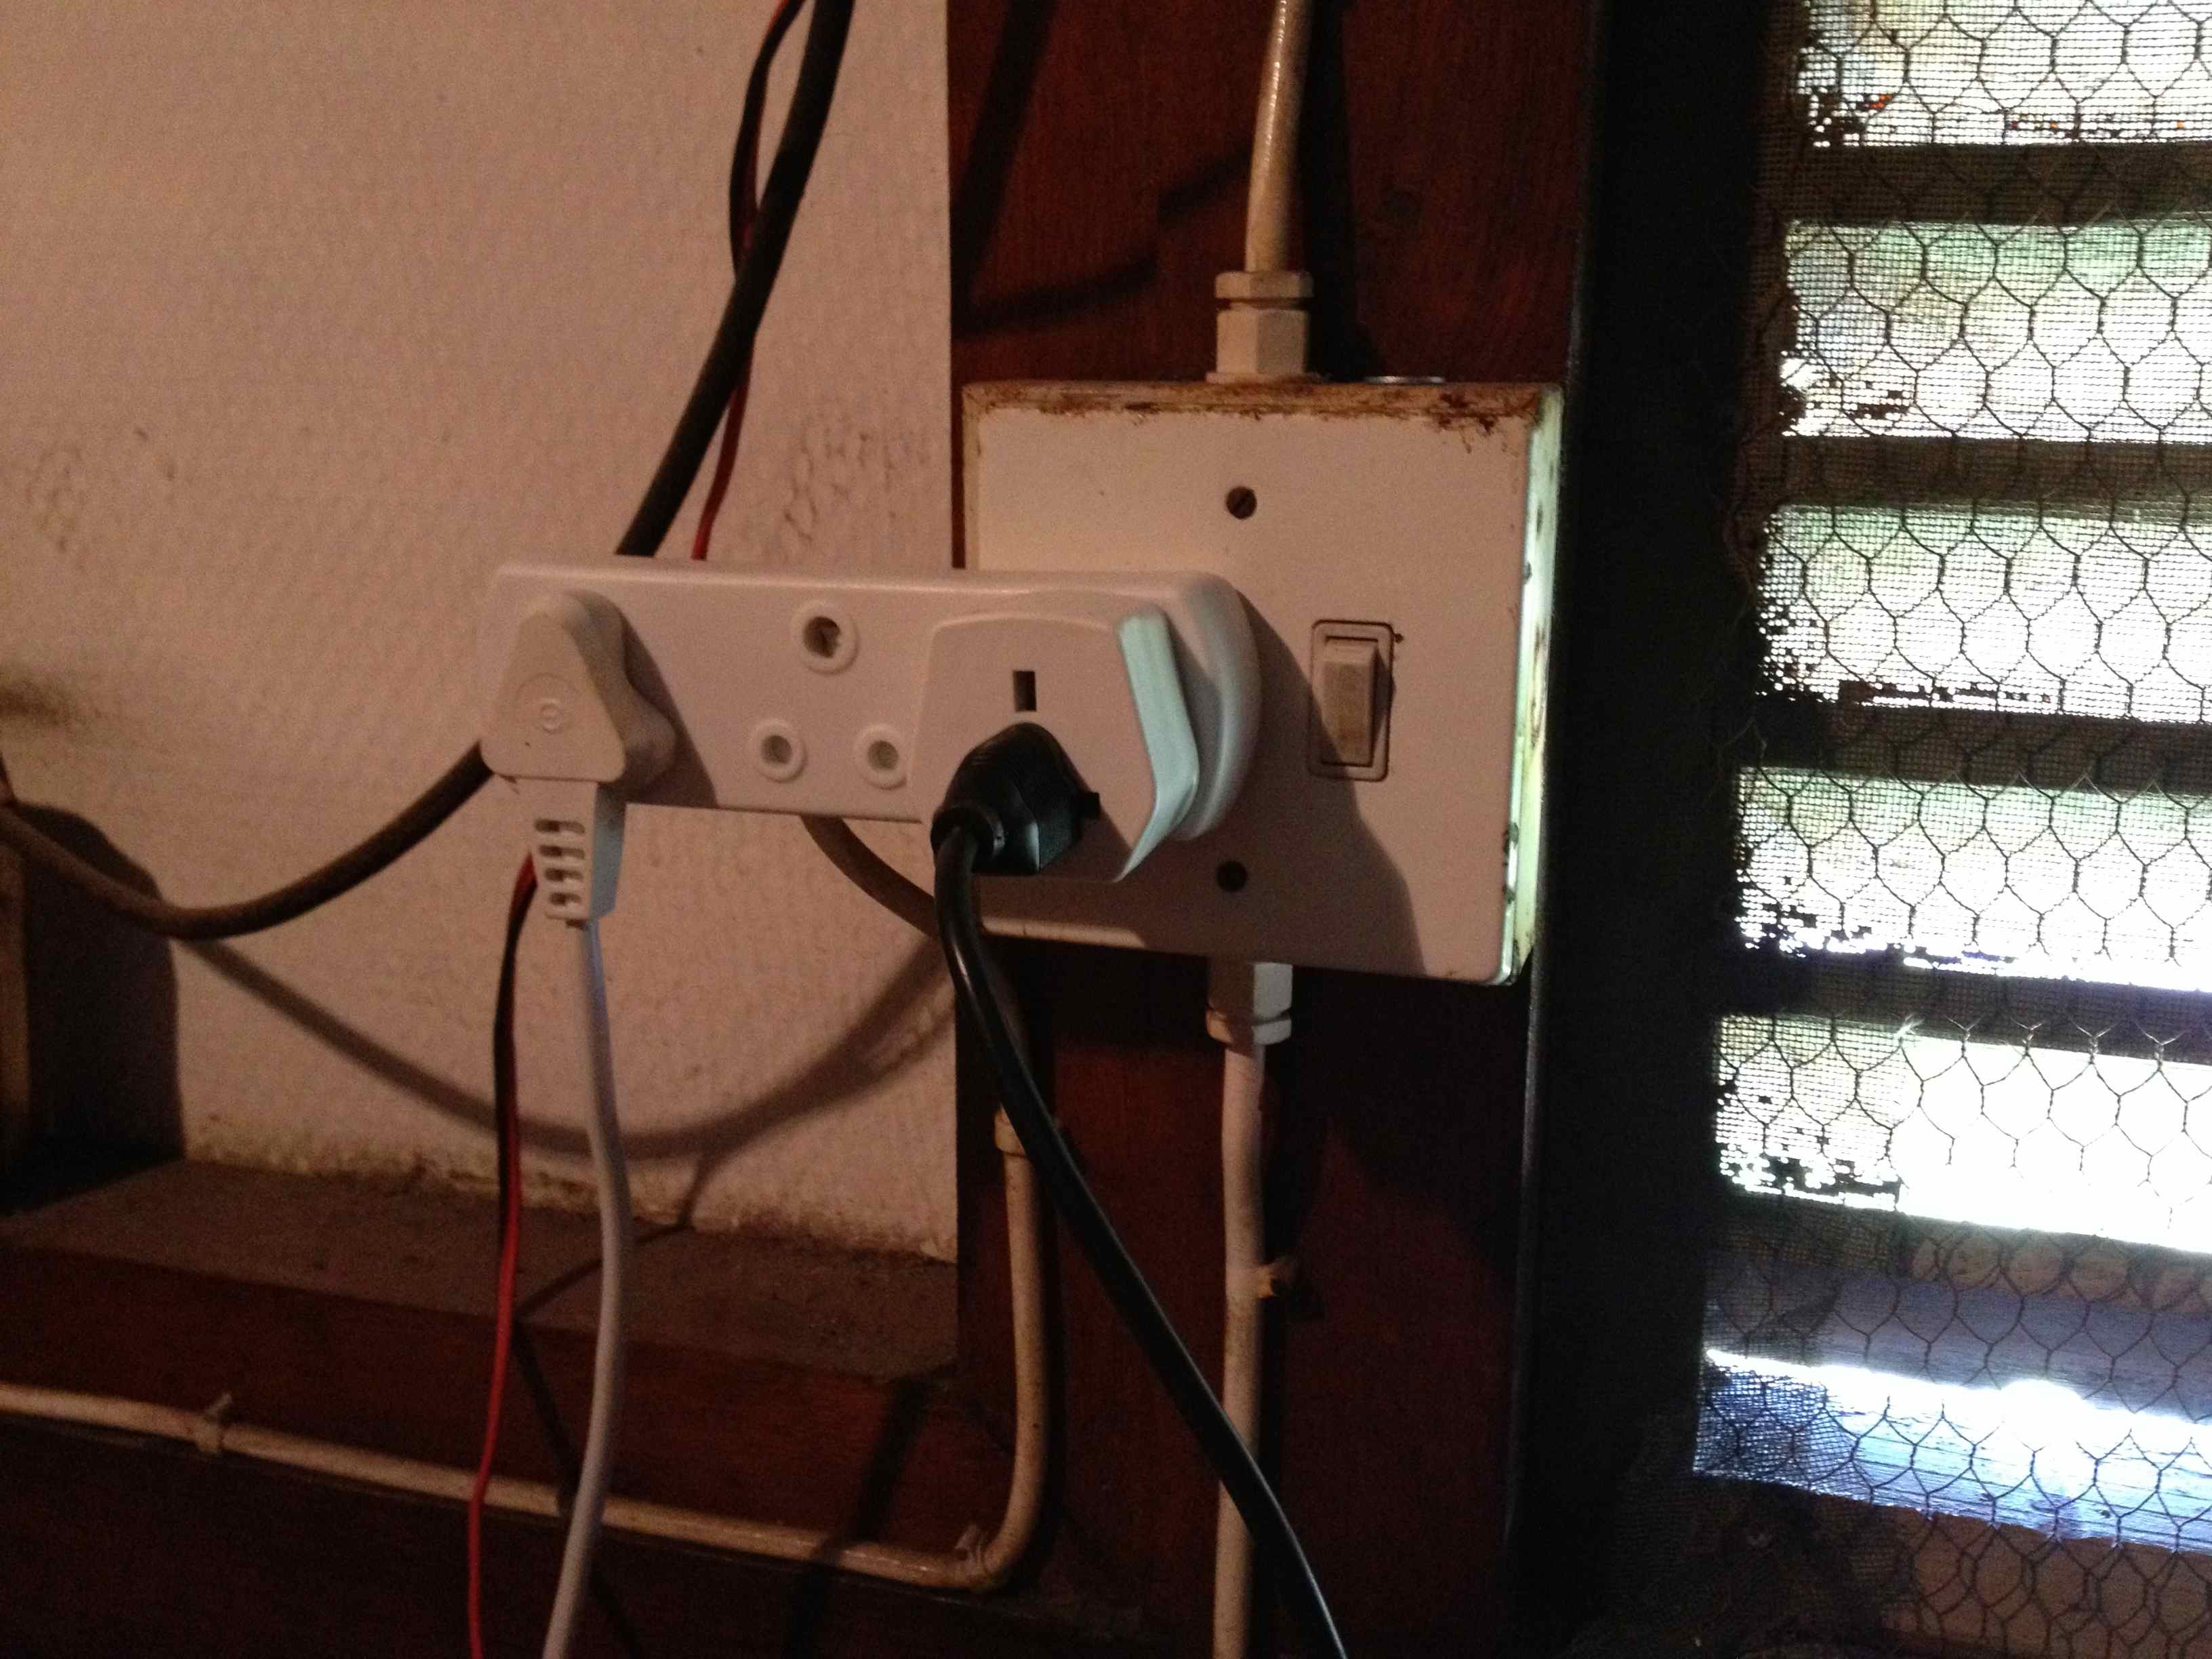
\includegraphics[width=0.49\textwidth]{documentation_images/plugseast}
    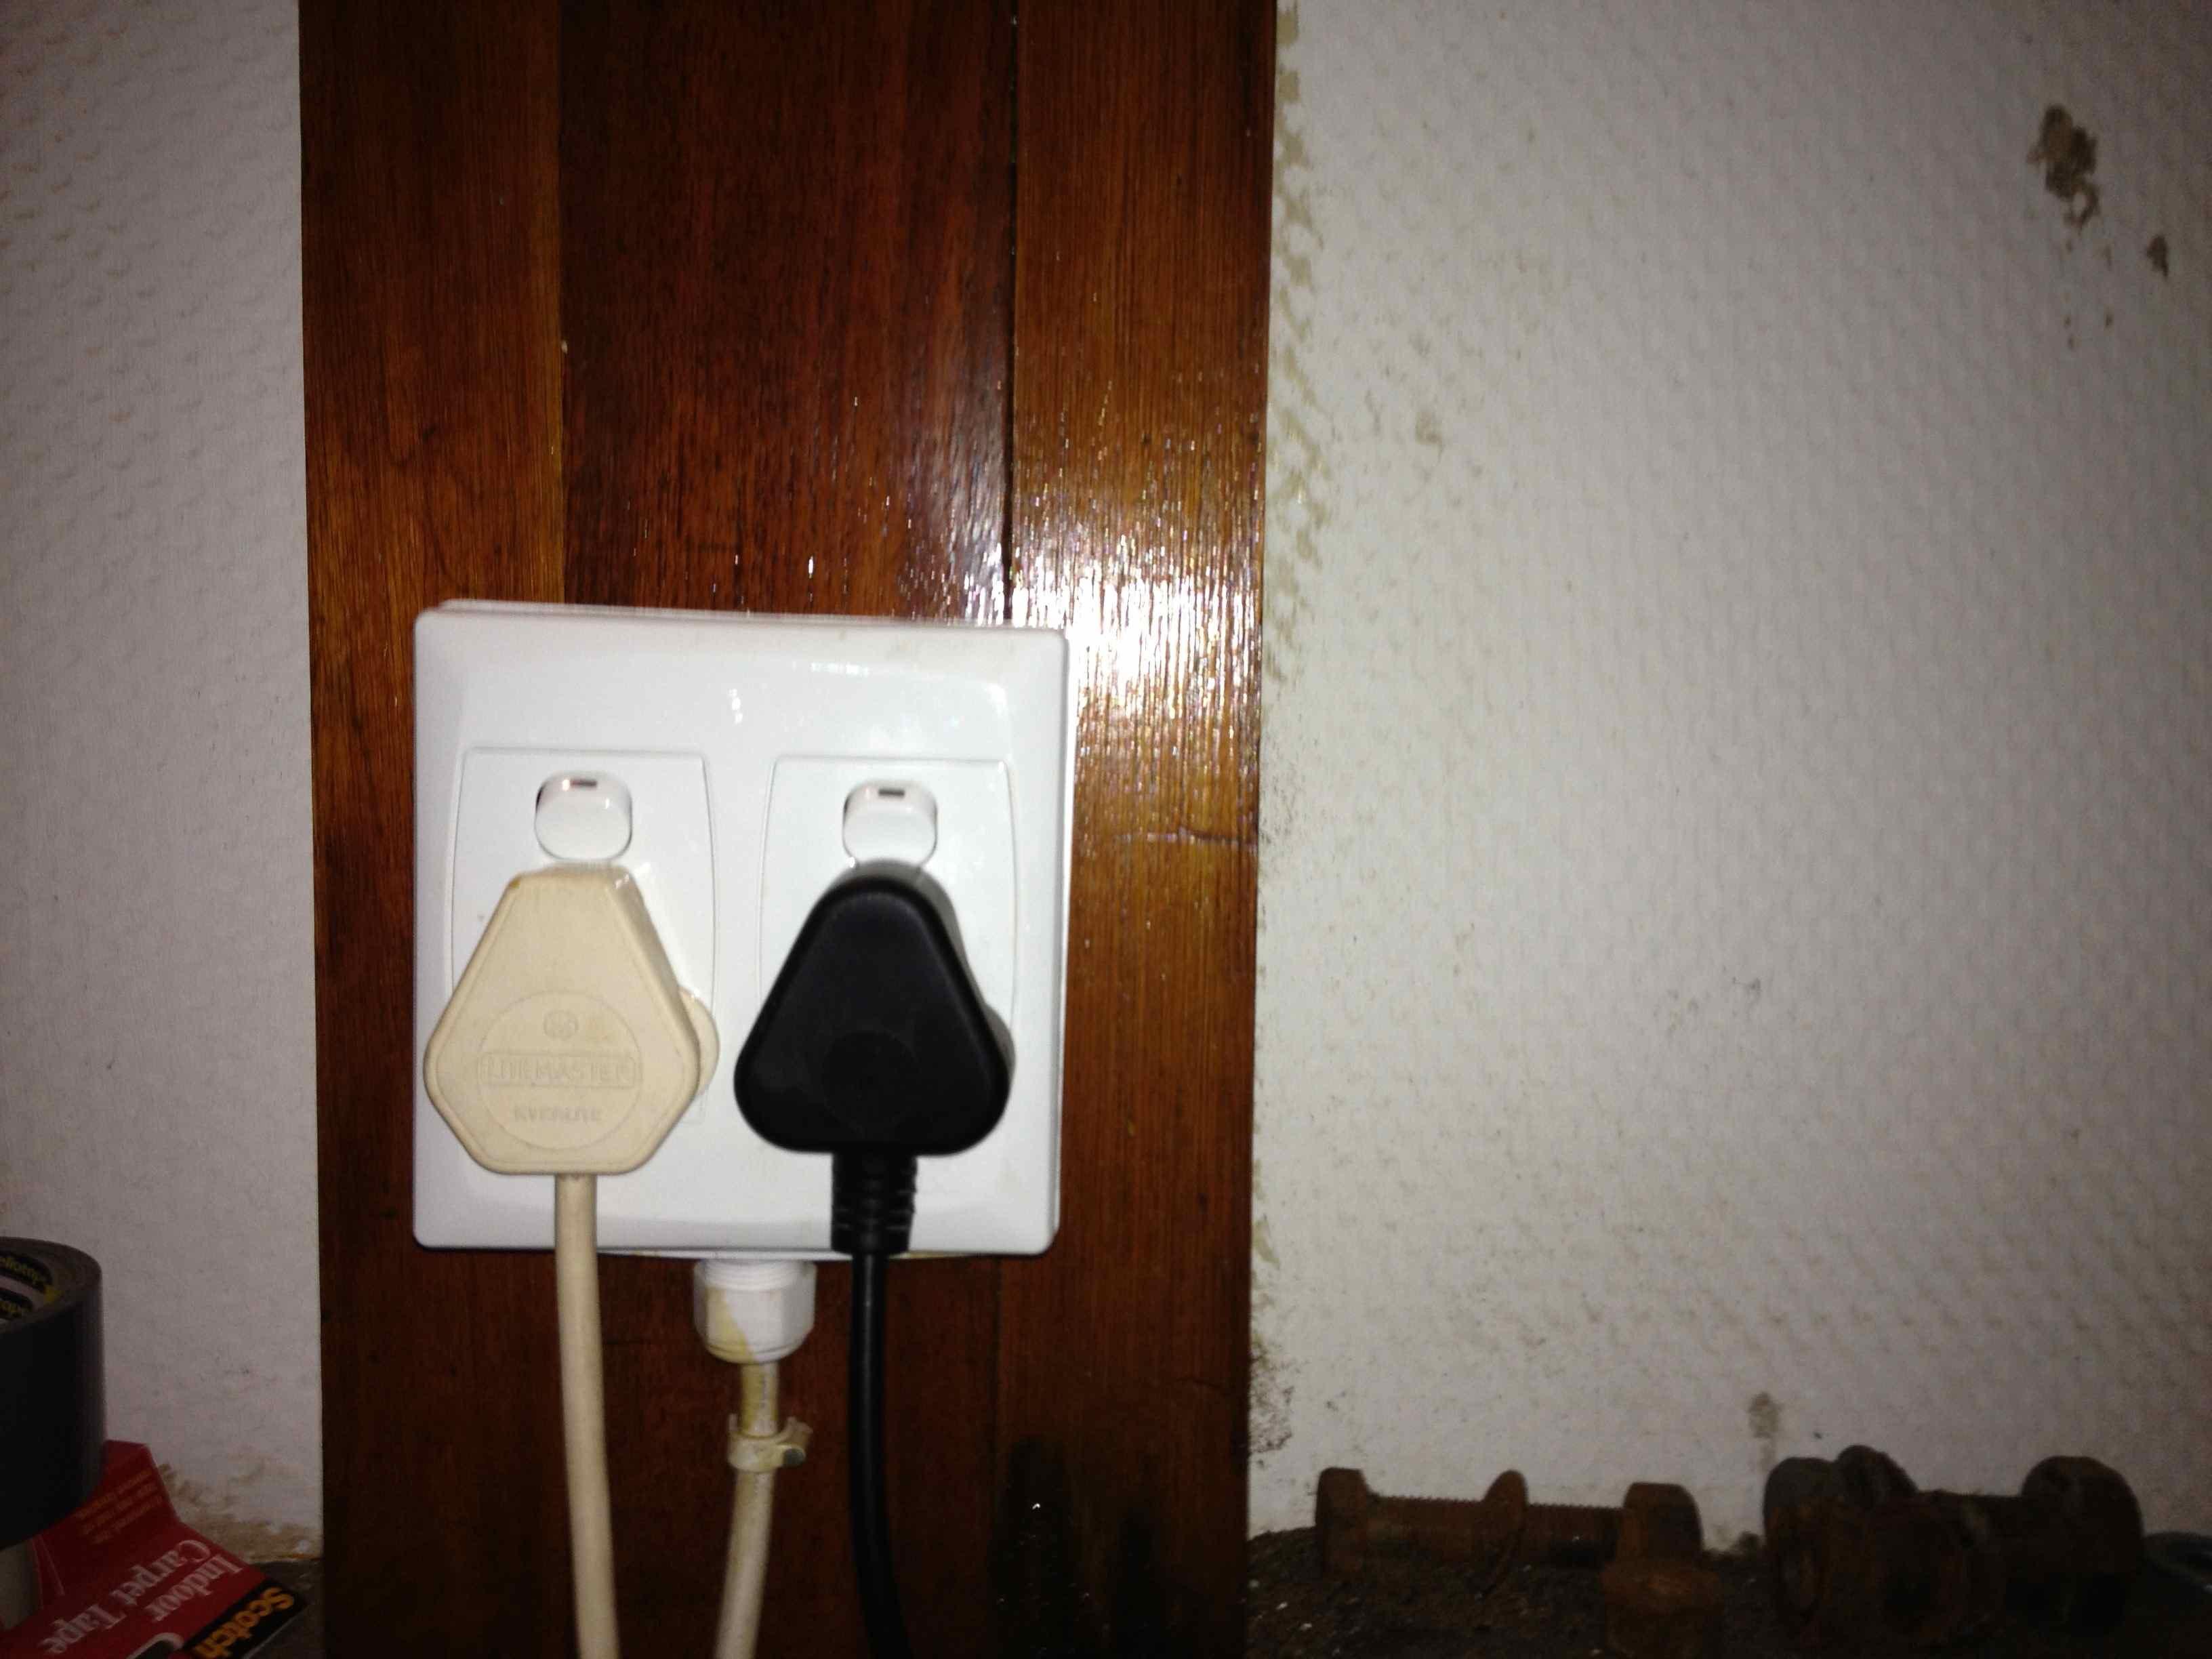
\includegraphics[width=0.49\textwidth]{documentation_images/plugsnorth}
    \caption{\label{fig:plugs} Switching on the power plugs. The left image shows the East wall plugs, the
image on the right shows the North wall plugs.}
\end{figure}


\subsection{Dome and telescope cover}

Currently, a sheet covers the telescope and protects it against dust. You can remove the sheet at this point.
In order to avoid damage to the telescope mirror from anything falling down whilst opening the dome, 
it is important to first open the dome (at present this requires a bit of elbow grease), after which 
you can remove the telescope cover. 

\subsection{Unlocking the RA and DEC drives}

When the telescope is parked during the day, both the Right Ascension (RA) and Declination (DEC) drives are 
in a 'locked' position, ensuring the telescope does not move when there is no power to the telescope.
At this stage of your observing session, you now need to put the RA and the DEC drive from a 'locked' position
to a 'star' position. This enables the telescope drive to be controlled from the laptop. 
Notice that when the drive clamps are in the mid position (marked by a 'balance' sign), the telescope 
can move freely. Be careful to gently hold/support the telescope when you switch the drives from 
lock to star position!

\begin{figure}[ht]
 \centering
    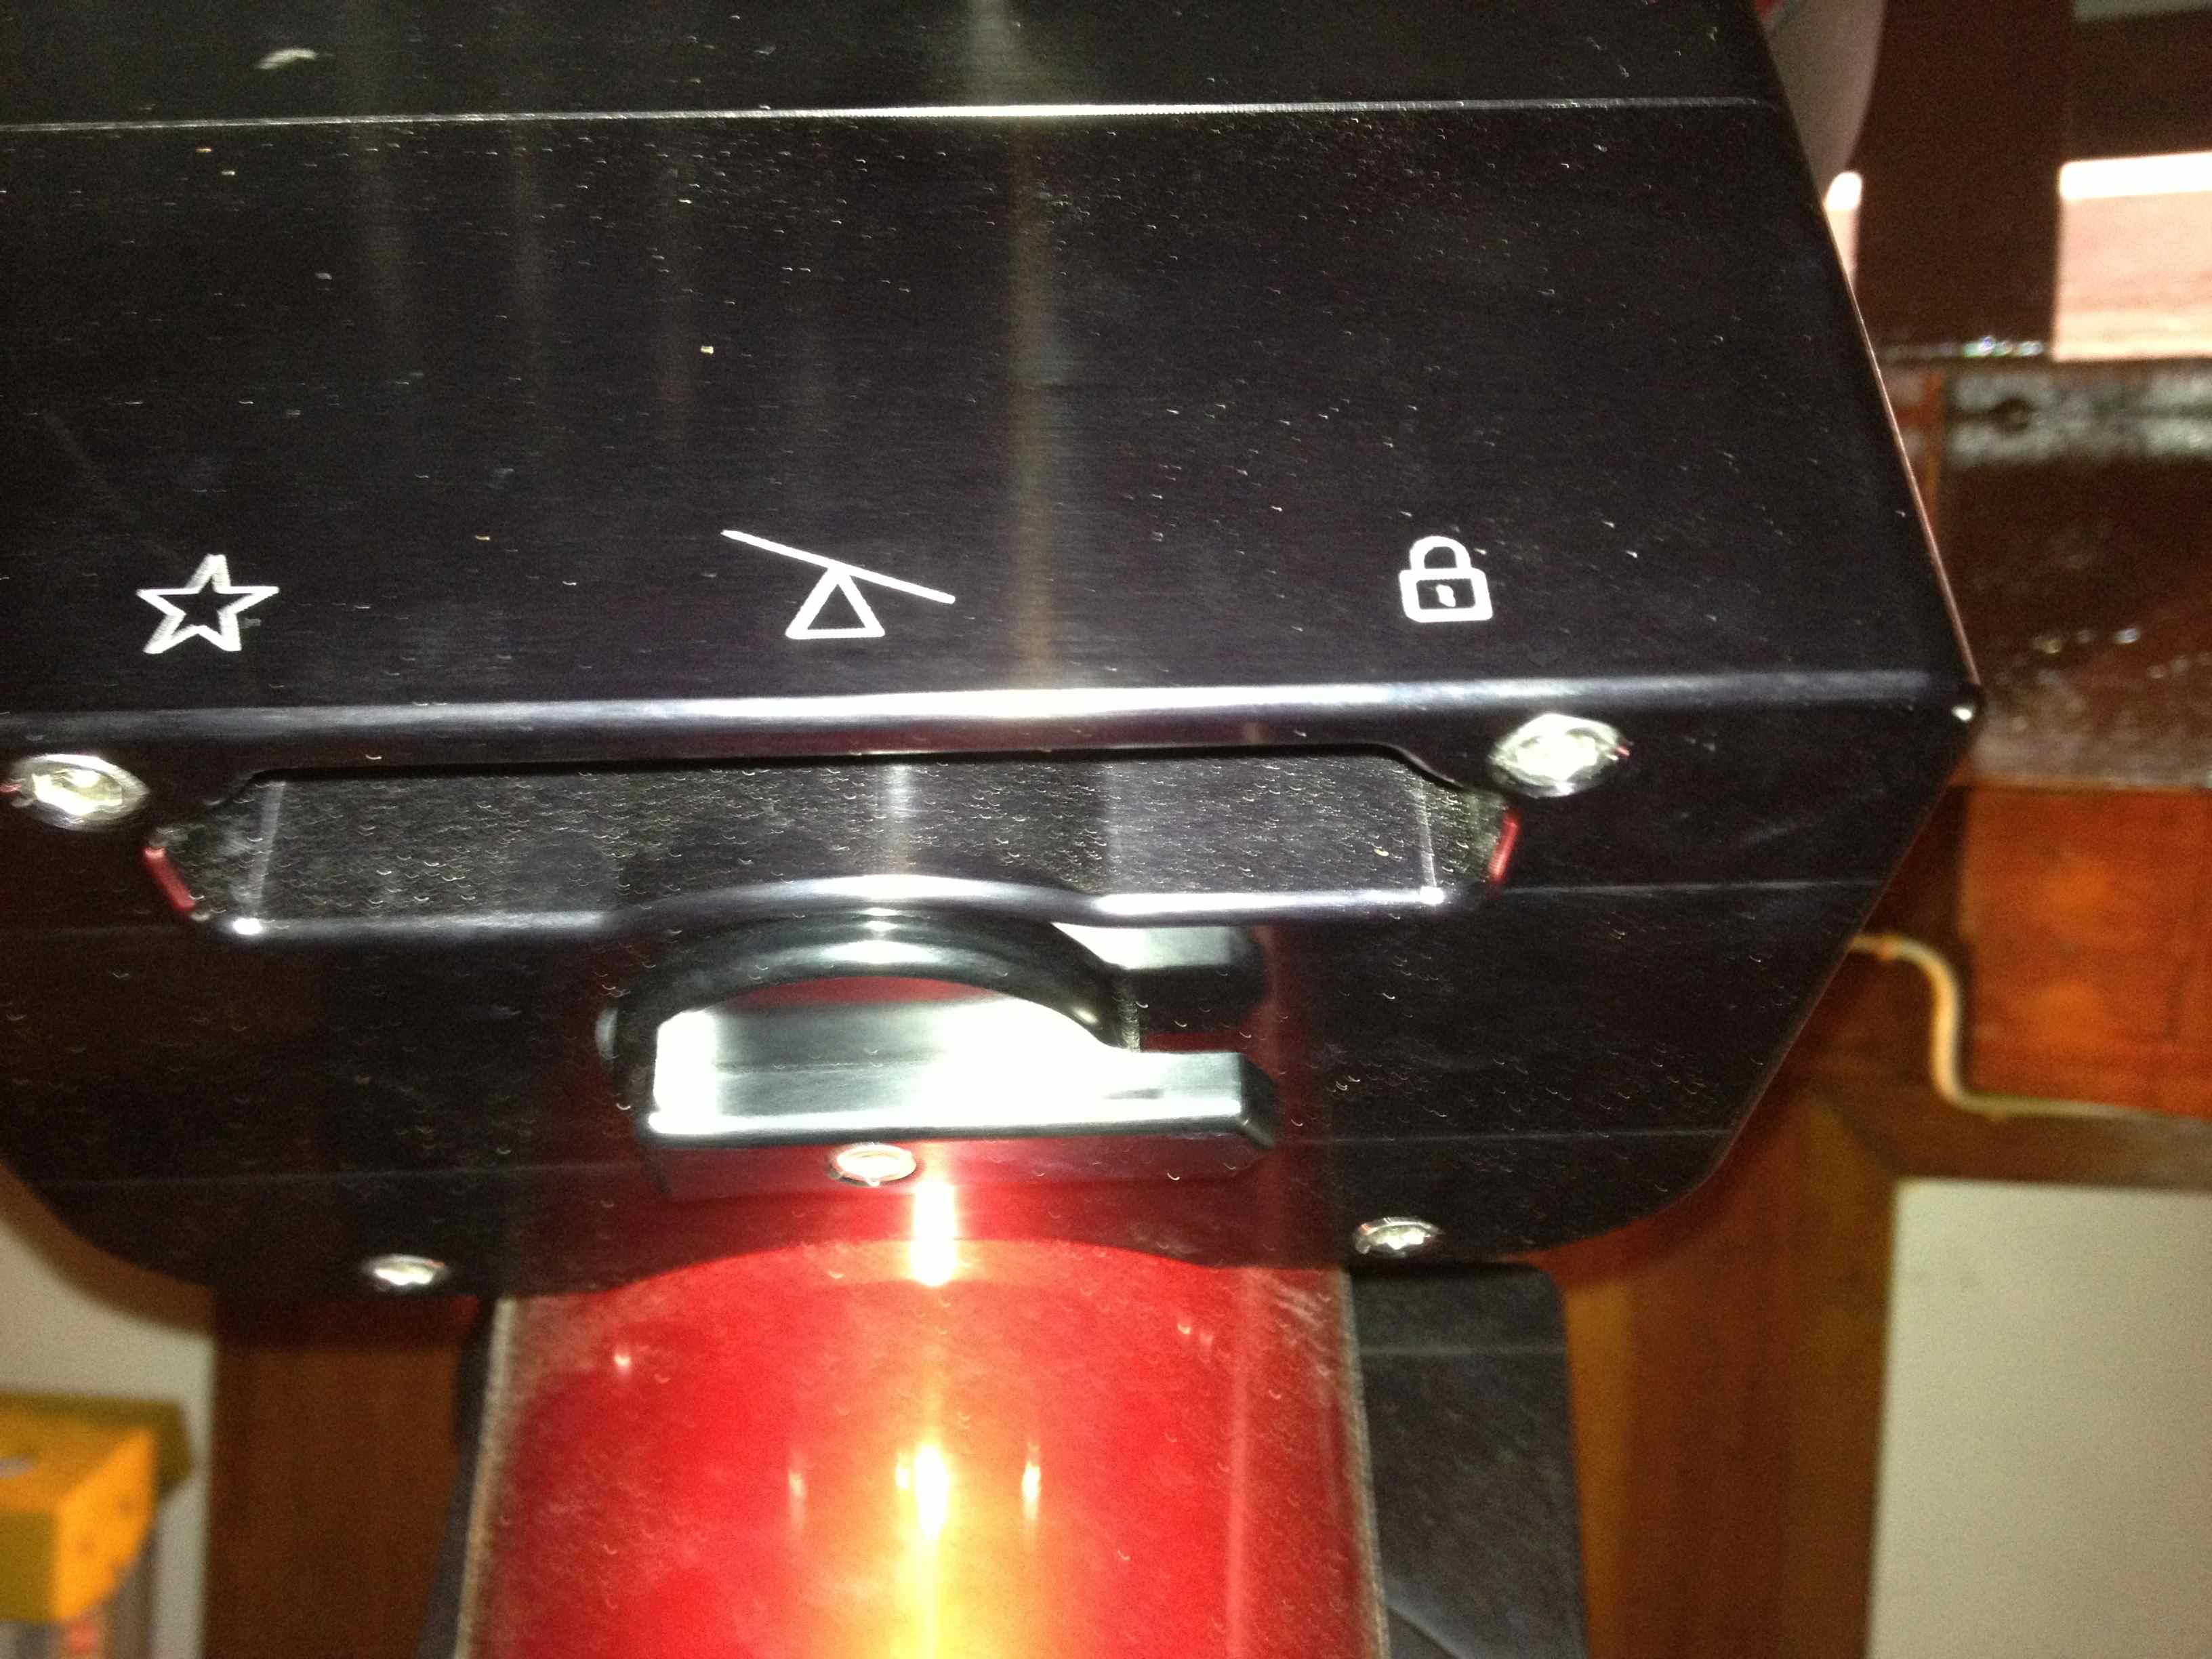
\includegraphics[width=0.49\textwidth]{documentation_images/decdrive}
    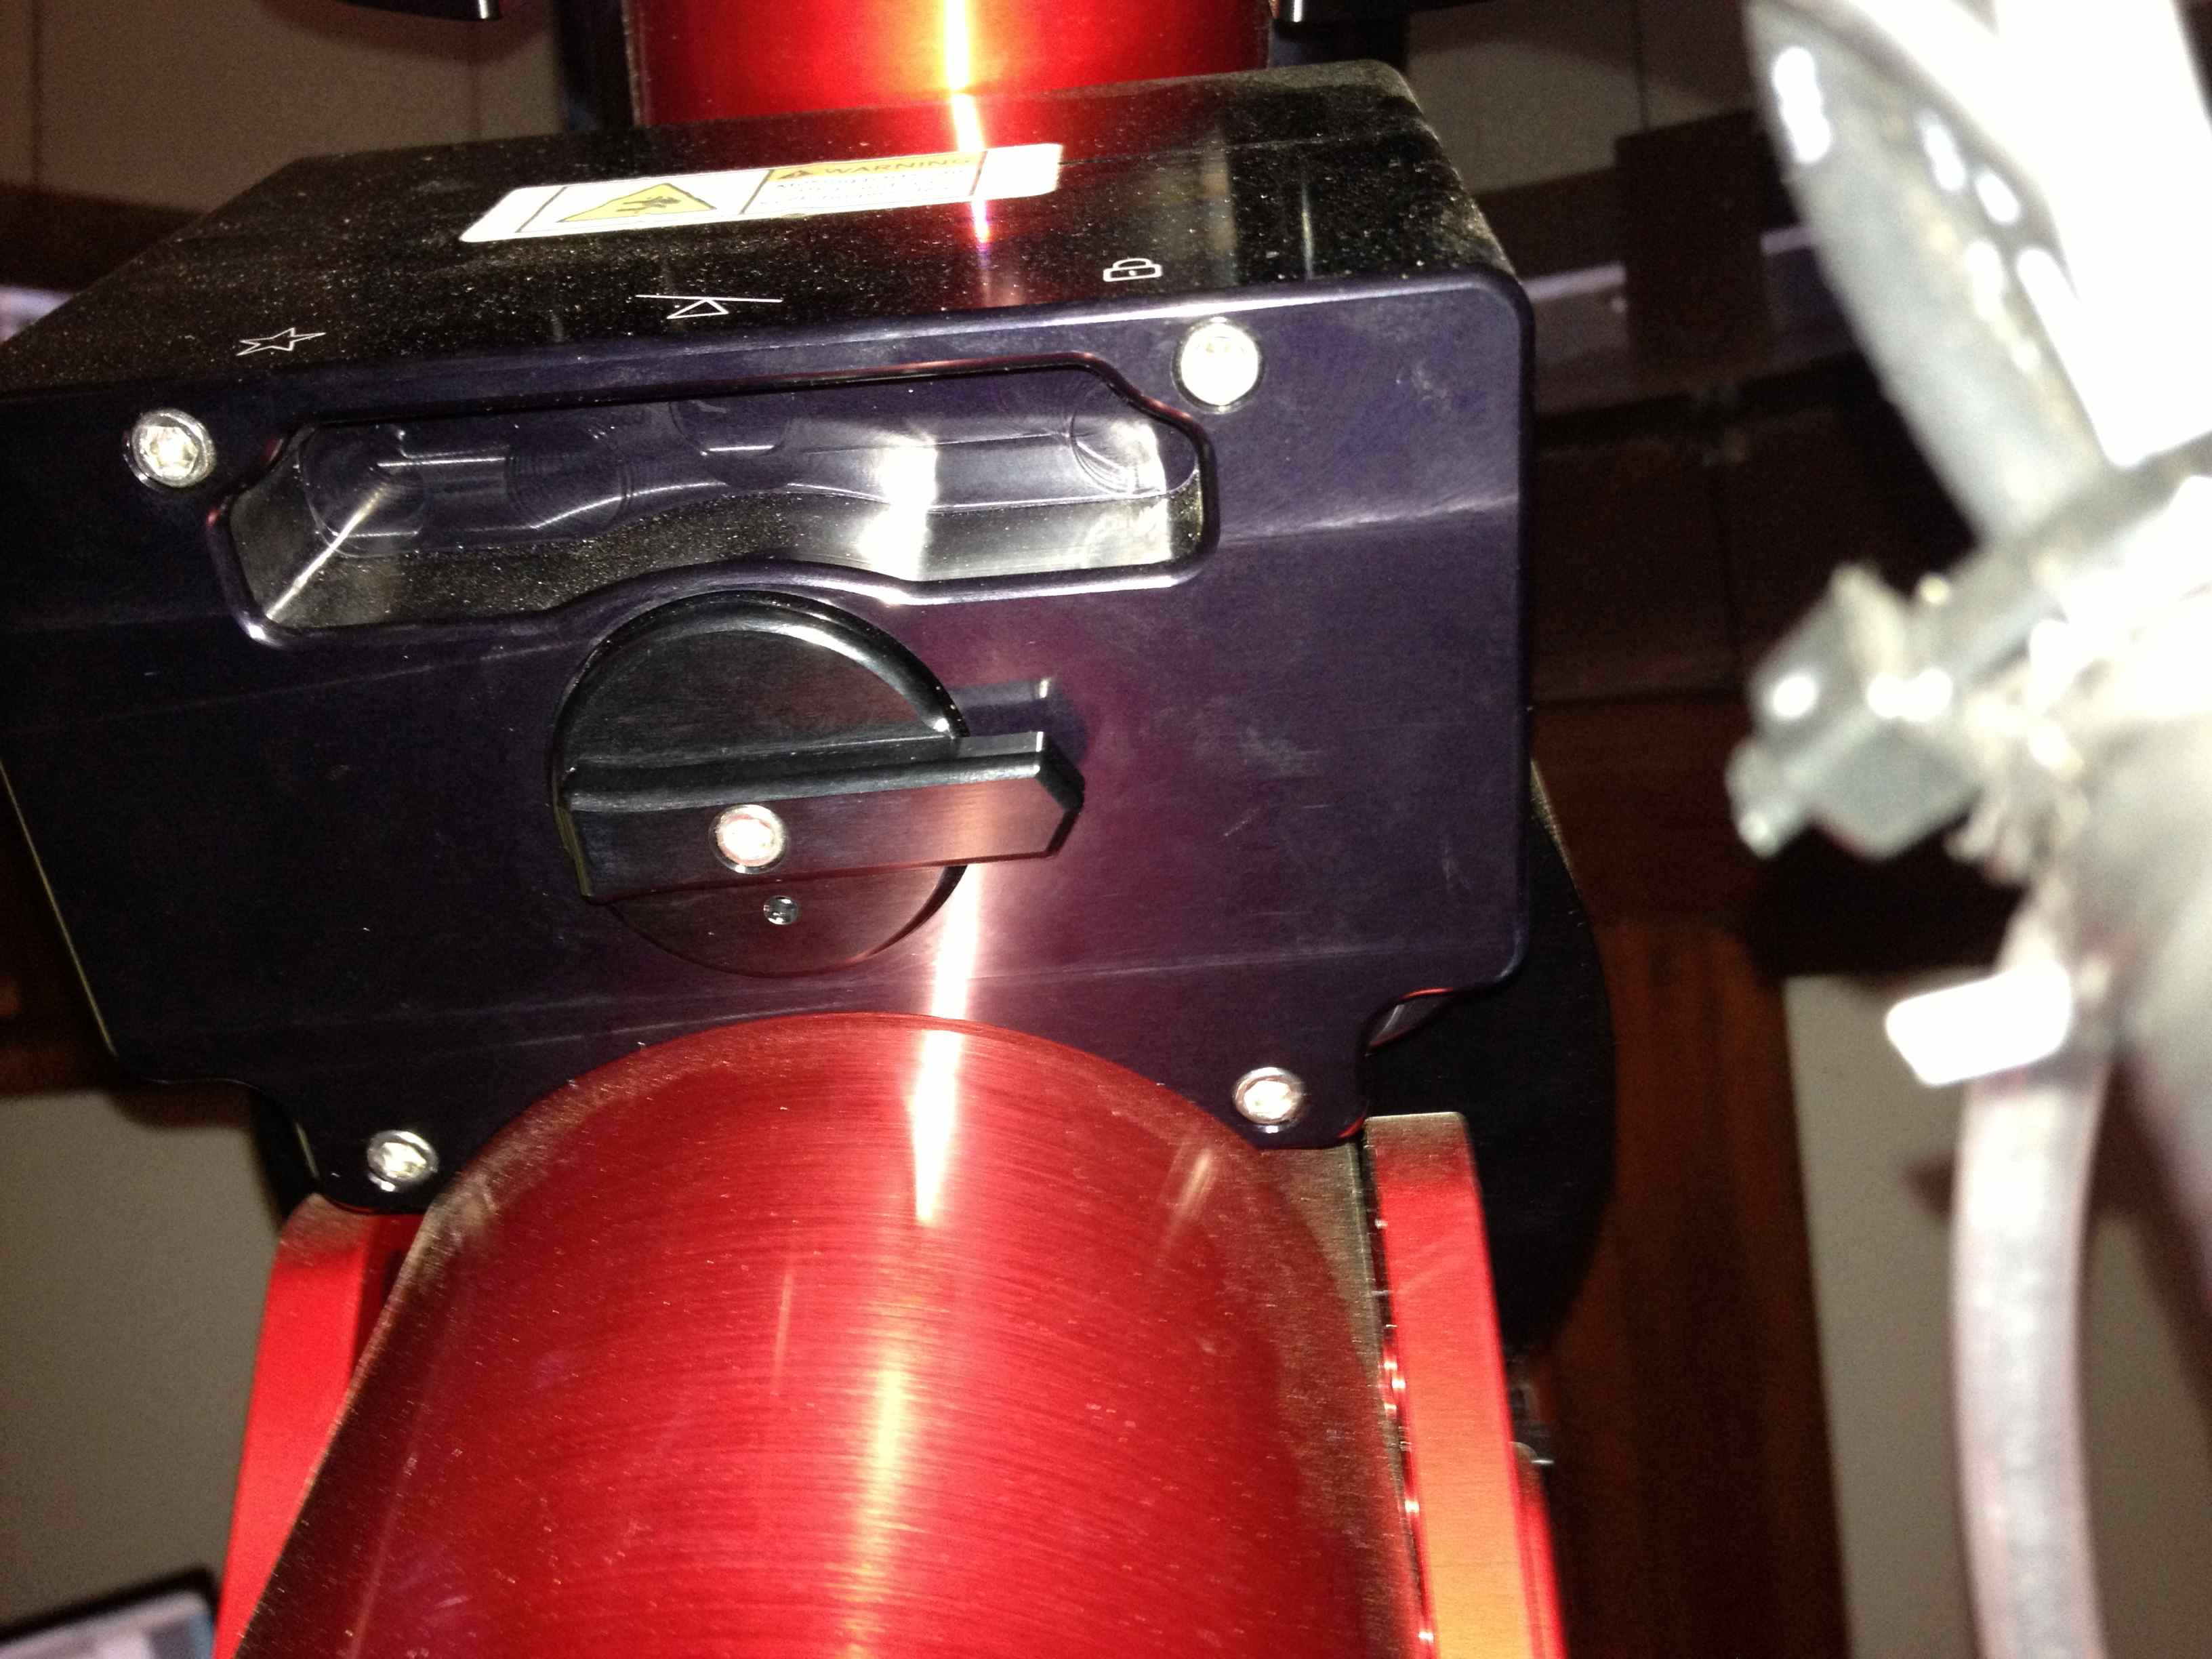
\includegraphics[width=0.49\textwidth]{documentation_images/radrive}
    \caption{\label{fig:drives} Left: Declination drive, right: Right Ascension drive.}
\end{figure}

\subsection{Telescope control: \emph{The SkyX}}

\emph{The SkyX} is an all inclusive astronomy program, that gives you the power of the 
universe at the point of a mouse. It should be able to guide the telescope, control the CCD, 
focus the image, control the dome and control the rotator. 
Unfortunately, it has some bugs so all it can really control at the moment the telescope, the 
dome rotation and the CCD rotator. To access the user manual for \emph{The SkyX}, 
visit \url{http://www.bisque.com/help/TheSkyXSAEAndPro/index.htm}.\\

On the laptop you can start \emph{The SkyX}. This program controls the telescope, the dome and the
rotator (on which the CCD is mounted).
You will see a big X symbol on the laptop for 'The SkyX Professional Edition'. Double click this
system to start \emph{The SkyX}. You can minimize the window during the observations if you need to 
toggle between telescope control and CCD control. You can reopen the window by clicking on the 'X' 
on the bottom bar.\\

During the start up procedure you need to \textit{connect} and \textit{find home} for the dome, 
the telescope and the rotator. 
To 'connect' the telescope, click on the \textbf{Telescope} bar on the left-vertical menu, and 
under the \textbf{Start Up} pull-down menu, select \textbf{Connect}. The program will then request 
a \textit{find home} procedure, which will initialise the telescope. Before you enable the 
\textit{find home} procedure, make sure to remove any chairs or obstacle that might be in the
way of the telescope as it move. Confirming the \textit{find home} command, will move the telescope 
to its start-up position. The status should read: {\textcolor{PineGreen}{\tt Tracking at sidereal rate}}.
The display of \emph{The SkyX},  \textit{connecting} the telescope is shown in 
Figure~\ref{fig:connect_telescope}.\\

\begin{figure}[ht]
 \centering
    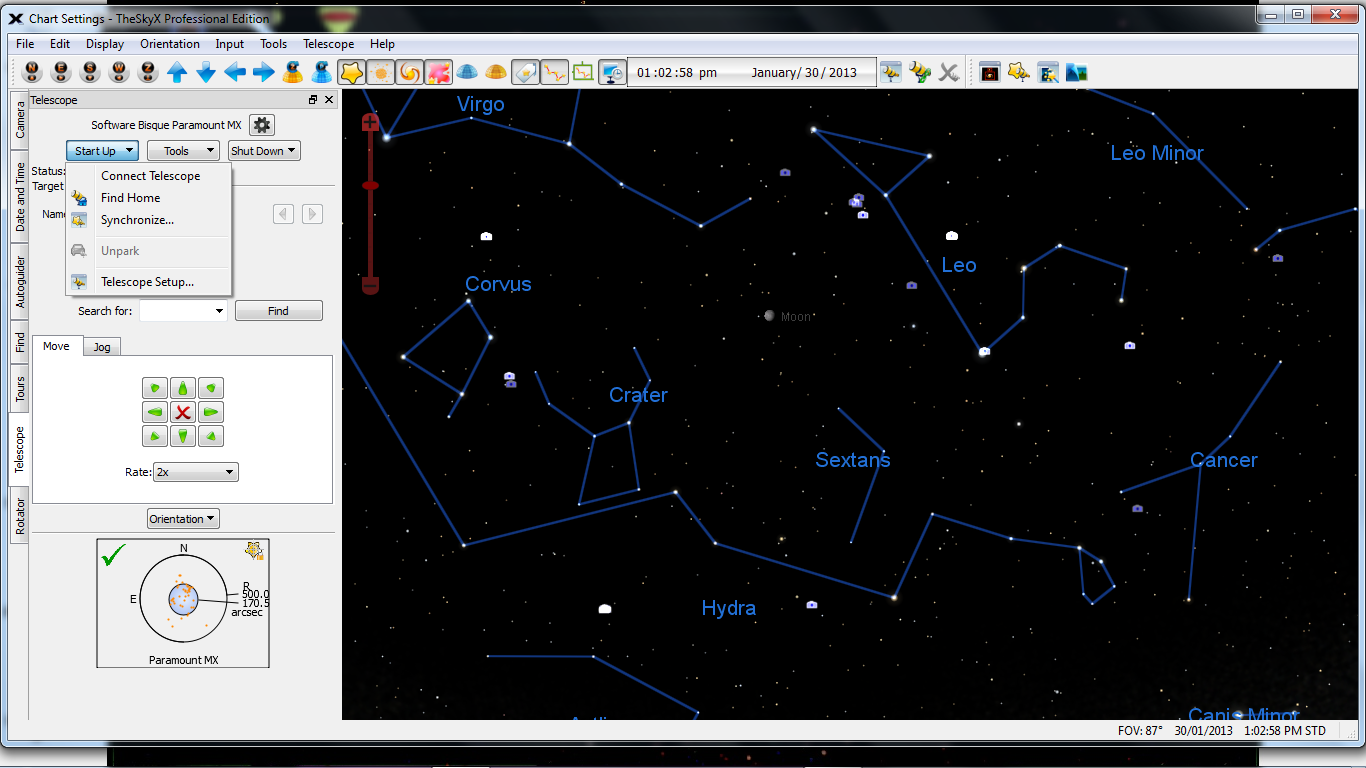
\includegraphics[width=\textwidth]{documentation_images/connect_telescope.png}
    \caption{\label{fig:connect_telescope} Shows how to connect the computer to the telescope.}
\end{figure}

To \textit{connect} the Dome, click on the \textbf{Dome} bar on the left-vertical menu and press 
\textbf{Connect}. The status of the Dome should now read: \textcolor{PineGreen}{\tt Connected}.
To \textit{connect} the rotator, click on the \textbf{Rotator} bar on the left-vertical menu and 
click \textbf{Connect}. Repeat this if \emph{The SkyX} complains.  The status of the Rotator should 
read: \textcolor{PineGreen}{\tt Ready}. The telescope is now ready for use.

\subsection{CCD control: \emph{Maxim DL}}

On the laptop you can start \emph{Maxim DL}. Double click on the symbol for 'Maxim DL Pro 5'. 
Minimisation of the window is the same as for \emph{The SkyX}.\\

To enable CCD camera control from the laptop, click on the \textit{Toggle Camera Control (CTRL + W)} button.
This button is located in the second row of the menu bar and looks like a 'button with two wires'. 
This will open a new window (entitled: camera control, see Figure~\ref{fig:coolers}).  
In this window, click \textbf{Connect}. 
A new window is launched (entitled: SBIG AO Control). On the 'camera control' window, click on
coolers \textbf{On}. This will cool the CCD camera. You will notice that the temperature for 
Camera 1 (the normal CCD) will drop to $-5$ C (a preset temperature that depends on the outside 
temperature).\\

\begin{figure}[ht]
 \centering
    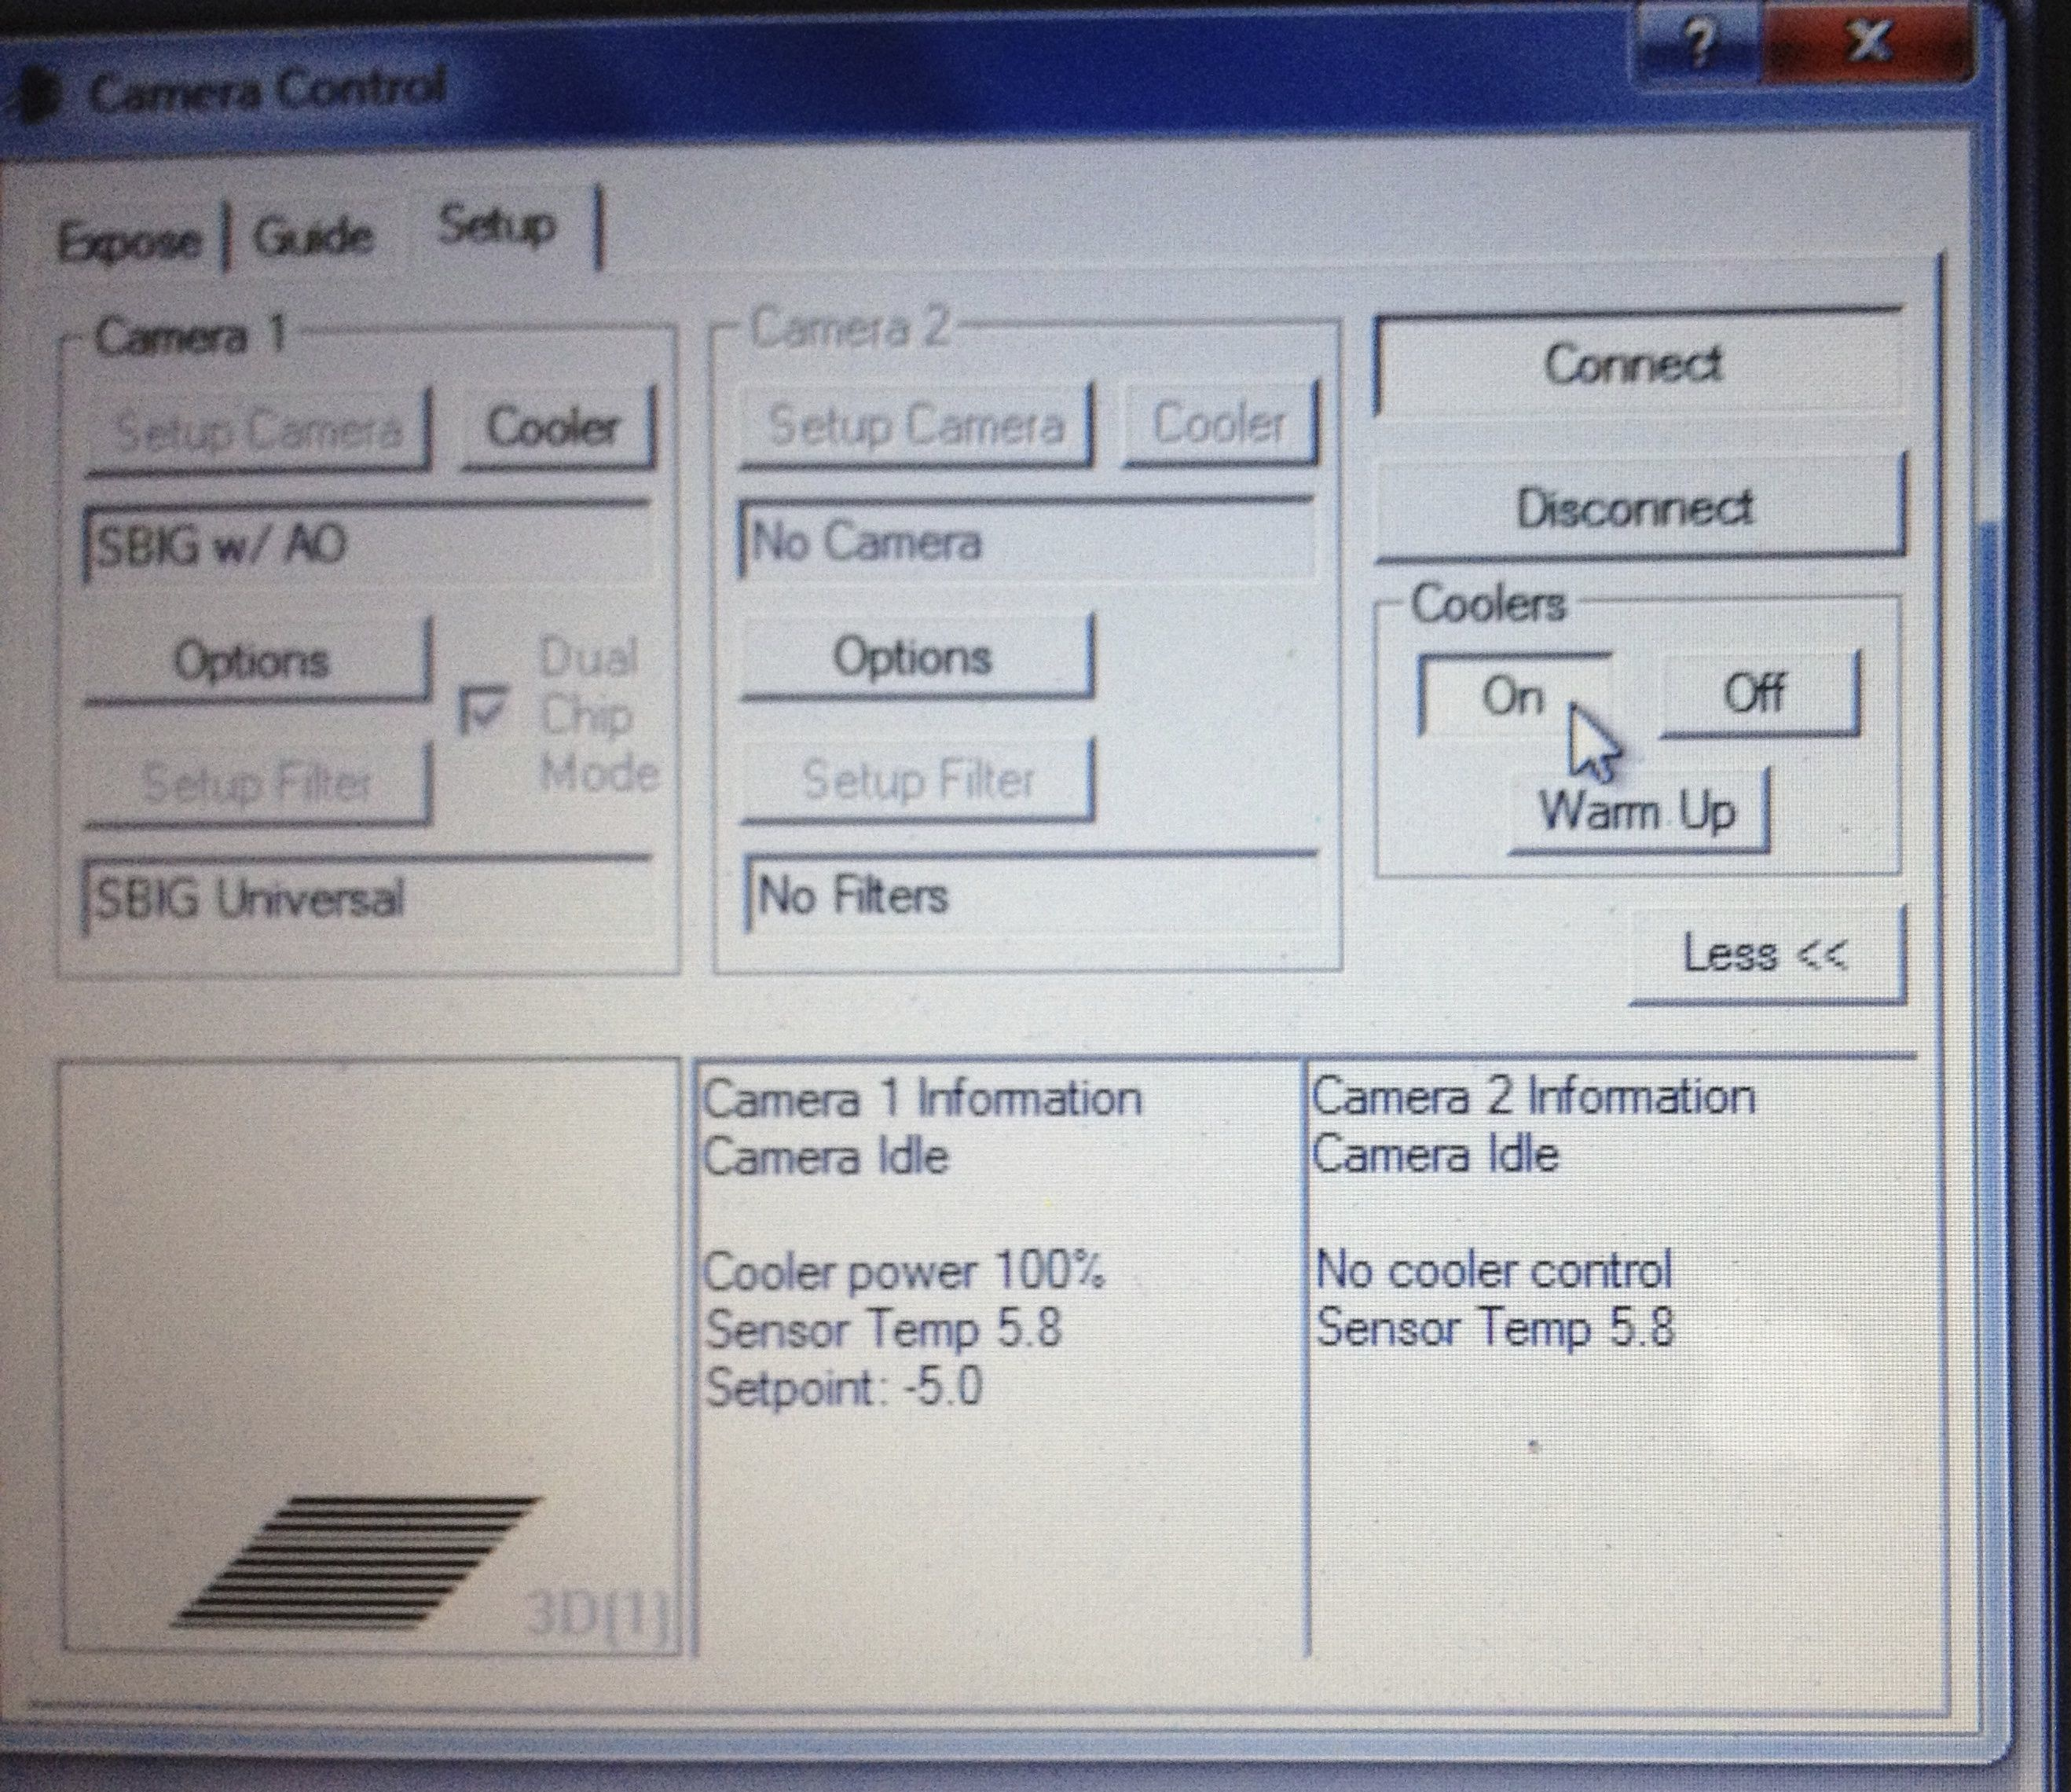
\includegraphics[width=0.49\textwidth]{documentation_images/maximdl_cooler}
    \caption{\label{fig:coolers} The camera control window on \emph{Maxim DL}.}
\end{figure}

Once the sensor temperature is down to the setpoint temperature, the CCD camera is ready for use. 
The cooling power should be around 60-70\%. If it is persistently above 70\%, change the setpoint 
temperature to a higher value (in steps of 5 C) through the 'Setup' button.\\

The entire system is now ready for on-sky observations, to align the pointing of the telescope and
to set the focus of the telescope. From there you can acquire your science target and set up the 
auto-guiding using the 'Adaptive Optics' module (Camera 2 on \emph{Maxim DL}). This is described
in the following two sections.



\section{Acquiring a target}
\label{acquire}

%\begin{figure}[h]
% \centering
%    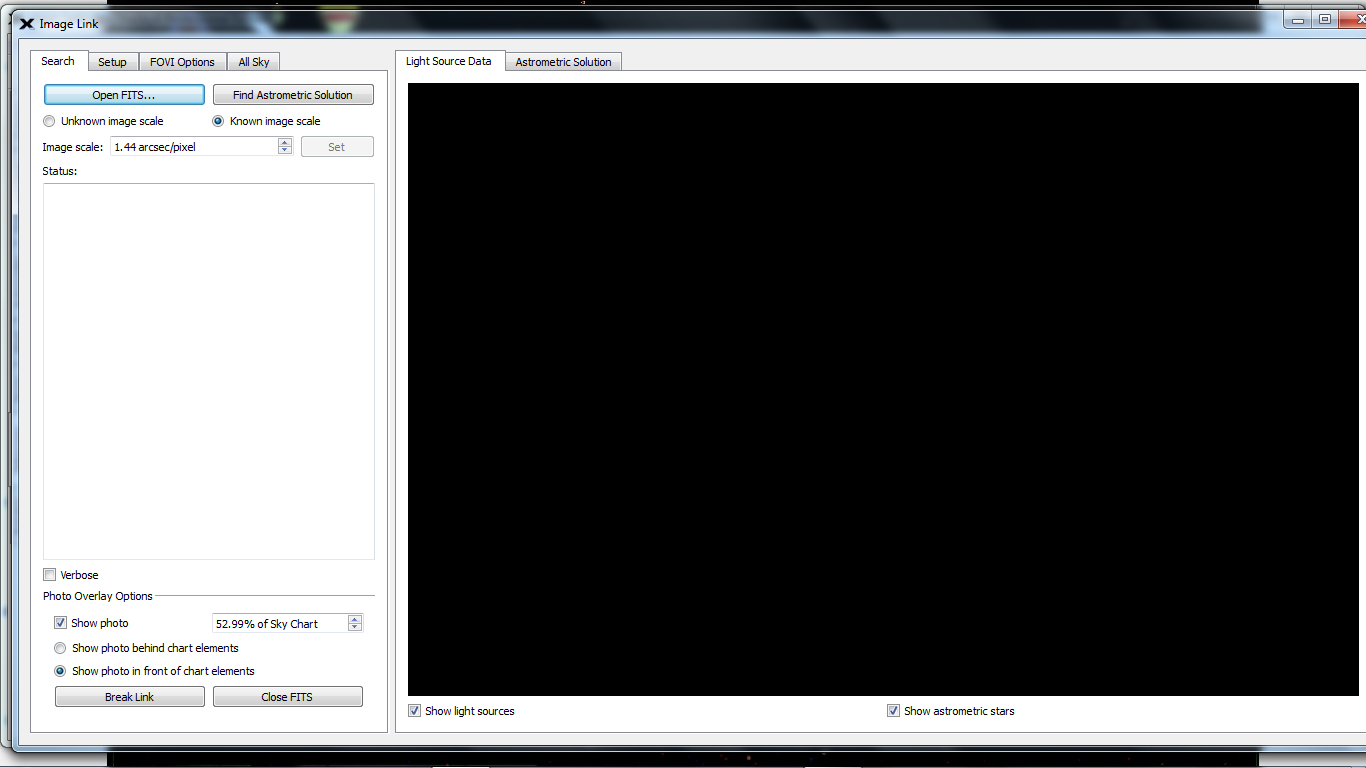
\includegraphics[width=\textwidth]{documentation_images/basic_interface.png}
%    \caption{\label{fig:basic_interface} This is how \emph{The SkyX} looks like when it is open.}
%\end{figure}

\subsection{Aligning the pointing of the telescope}

\subsection{Focussing the telescope}

\subsection{Selecting a guide star}


%\subsection{Small Changes to Pointing}
%\label{small_changes_to_pointing}
If the pointing of the telescope is off, follow these steps to correct it.
\begin{enumerate}
 \item Slew to field you would like to be look at.
 \begin{figure}[h]
 \centering
    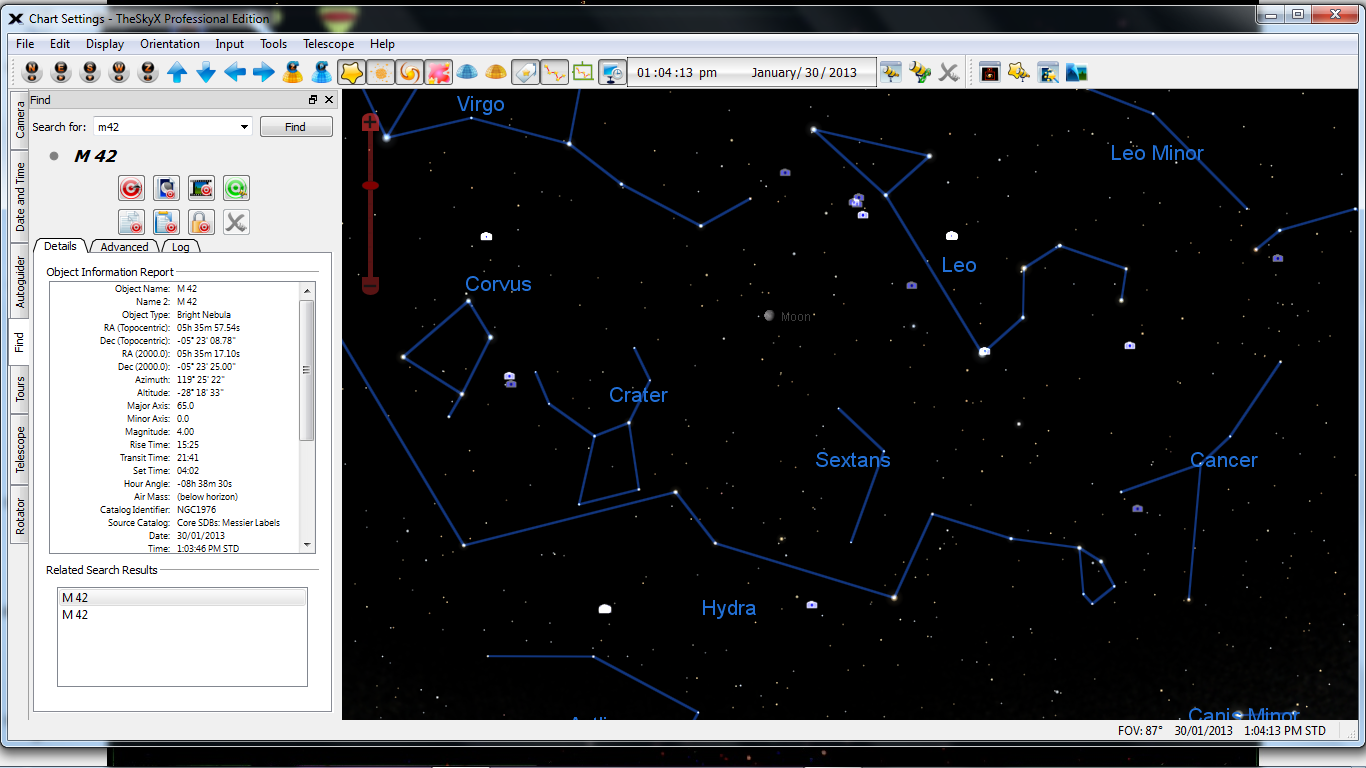
\includegraphics[width=\textwidth]{documentation_images/moving_telescope.png}
    \caption{\label{fig:moving_telescope} Click the green slew button to start the telescopes movement.}
\end{figure}
 \item \label{2} Take an image with your favorite CCD manager and save it.
 \item In \emph{The SkyX}, under the menu tools--Image link (Ctrl+Shift+I), in the Search tab, click the \emph{Open FITS...} window.
  \begin{figure}[h]
 \centering
    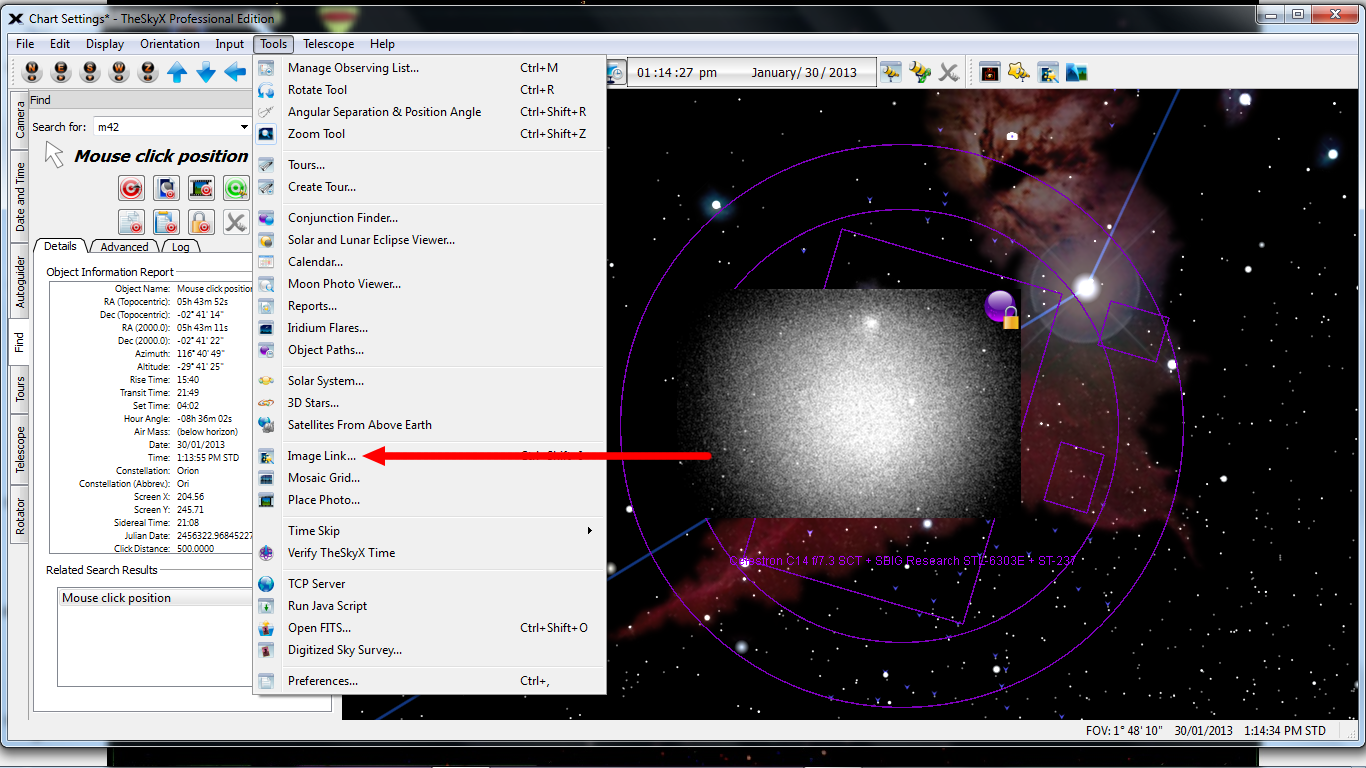
\includegraphics[width=\textwidth]{documentation_images/tools_menu_1_1.png}
    \caption{\label{fig:tools_menu} Click at arrow to access image linking window.}
    \end{figure}
    
  \begin{figure}[h]
 \centering
    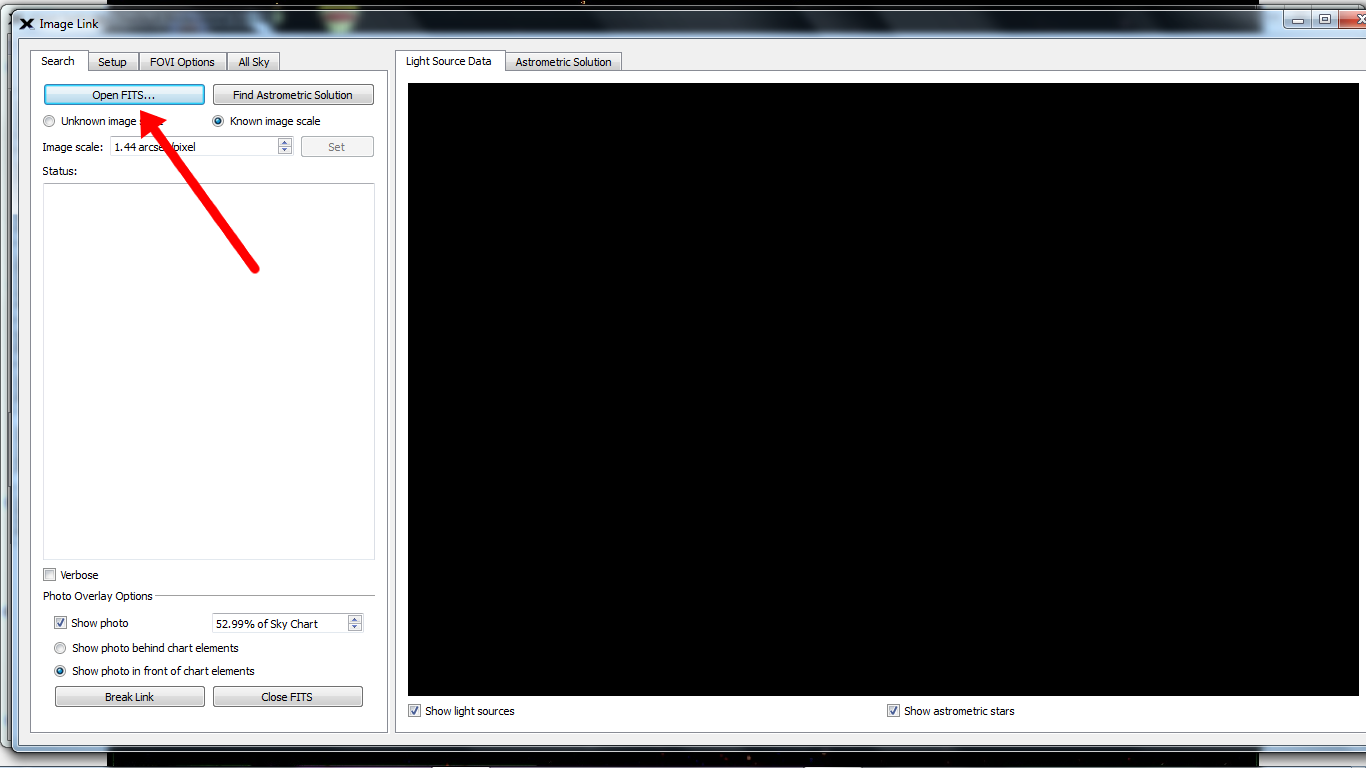
\includegraphics[width=\textwidth]{documentation_images/pointing1_1.png}
    \caption{\label{fig:pointing1} Click at arrow to access image linking window.}
    \end{figure}

 \item Load in saved test field from step \ref{2} and then click the \emph{Find Astrometric Solution} button.
 \item If solution fails, check Image scale and binning of image they should be:
 \begin{itemize}
  \item $1\times1 = 0.72$ arcseconds
  \item $2\times2 = 1.44$ arcseconds
  \item $3\times3 = 2.15$ arcseconds
  \item $4\times4 = 2.88$ arcseconds 
 \end{itemize}
 \item Go to the \emph{FOVI Options} tab and click the \emph{Synchronize Rotator Angle to Position Angle} button.
  \begin{figure}[h]
 \centering
    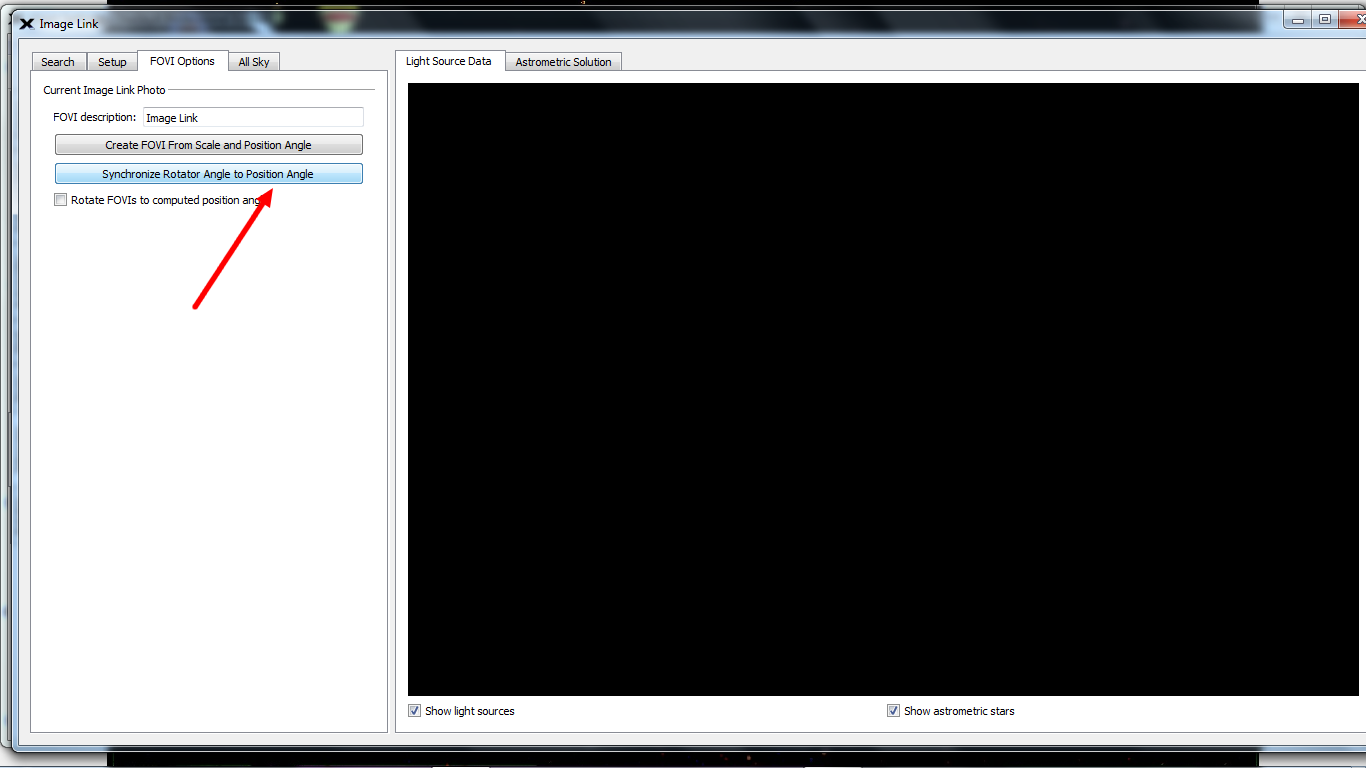
\includegraphics[width=\textwidth]{documentation_images/pointing2_1.png}
    \caption{\label{fig:pointing1} Click at arrow to access sync telescope pointing with image.}
    \end{figure}

 \item Exit from window and go back to the main screen.
 \item Click on Image until in the \emph{Find} tab shows Linked Photo.
 \item Click on the \emph{Sync} button on the tool-bar and it should be pointing in the correct direction now. If not repeat from beginning.
\end{enumerate}

%\subsection{Rotator}
%\label{Correcting_rotation}
\emph{The SkyX} can control the rotation of the camera, but there is a bug in the software that causes the readings to be off, and this changes depending on where you are pointing in the sky. There is also no easy way to adjust the rotation of the CCD in \emph{The SkyX}.

The rotator is important for selecting a guide star for the Adaptive Optics (AO). The following steps tell you how to calibrate and align a guide star on the AO CCD.
\begin{enumerate}
 \item 
\end{enumerate}


%\subsection{Remote Observations}
%\label{remote_obs}


%\subsection{Dome Control}
%\label{Dome_control}
%TBA
%\label{dome_position}



\vfill \eject 

\section{Science imaging}

\vfill \eject

\section{Close down procedures}

The close down procedure is the inverse of the start up process.

\subsection{CCD control: \emph{Maxim DL}}

On the camera control window (\emph{Maxim DL}), click on 'Warm Up' under ``Coolers'', and click 'Disconnect' once camera 1
indicates that the cooler control is off.

\subsection{Telescope control: \emph{The SkyX}}

On \emph{The SkyX}, select the 'Telescope' tab. Under the 'Shut Down' pull-down menu, select 'Park', to 
move the telescope to the park position (status should be green and read ``Parked''). 
Select the 'Dome' tab and select ``Park Dome'' to move the dome to the park position. Then select 
``Disconnect'' (status should change to red and read ``Not Connected'').
Select the 'Rotator' tab and select ``Disconnect'' (status should change to red and read ``Not Connected'').
Finally, under 'Telescope', and the 'Shut Down' menu, select ``Disconnect'' to disconnect the telescope (status
should change to red and read ``Not Connected''. The telescope is now parked.

\subsection{Locking the RA and DEC drives}

Change the RA and DEC drive clamps from the 'star' position to the 'locked' positions. 
Notice that the telescope will move a bit even when it is in the 'locked' position. Move the
telescope until it physically locks into the 'locked' position.

\subsection{Dome and telescope cover}

\subsection{Disconnect power}


\section{Check lists}
\label{checklists}

%If you want to get started at making images quickly and don't have the time to get into the nitty gritty details of astronomy 
%go to the next section.

\subsection{Start of Night Check List}

\begin{enumerate}
 \item Plug in observation computer to power, internet, Dome controller usb and Telescope controller usb and turn on switches in observatory.
 \item Open the dome and take off telescope cover.
 \item Put telescope mount from lock to star position on both RA and Dec controllers.
 \item Start \emph{TheSkyX} and \emph{Maxim DL} on the laptop.
 \item Connect observation computer to internet if wanting to use remote software (see \ref{remote_obs} for more information). 
 \item Make sure chairs and tables are not in the way telescopes movement.
 \item Connect dome control, rotation and mount control in \emph{TheSkyX}. Tell all to go to home position and start! 
See section \ref{Dome_control} for more information.
 \item Find star to focus (less than 7.5 - 9 magnitude star) using Focus Max.
  \item Fine tune dome position (see section \ref{dome_position}).
 \item Slew to object, select filter, check rotation and expose and get some coffee.
 
\end{enumerate}

%coffee stain
%\cofeAm{.1}{1.0}{0}{5.5cm}{3cm}

\subsection{End of Night Check List}


\begin{enumerate}
 \item Park telescope and Dome and disconnect all systems from computer.
 \item Turn off observation computer.
 \item Put mount from star position to lock position.
 \item Power off all power supplies in dome.
 \item Close the dome shutter.
 \item Put telescope cover over telescope.
 \item Get some sleep.
\end{enumerate}


\chapter{Advanced Observation Procedures}

\section{Remote observing}

\subsection{Remote access}

Sitting in the dome all night while the telescope integrates is generally not a good idea. 
The temperature differences between your body can cause differences in the seeing in the telescope. 
We have set up a way to access the telescope computer from a remote place, so that the disturbances 
of the telescope are kept to a minimum.

To get the remote control software, goto \url{http://www.teamviewer.com/en/} and install 
the software on your computer. To access the observatory computer use the address: 
{\tt telescope.ast.uct.ac.za} and password: {\tt Bonjour7}.

Make sure that in the observatory that the telescope wont run into anything 
as it move throughout the night. Sit back in your remote setting and regularly keep an eye 
on the weather conditions. 

\subsection{Weather conditions}

\section{Instrument change}

In the course of 2013, a spectrograph will be added to the suite of instruments
at the UCT Teaching Observatory. This section will describe how to change between
the CCD camera and the spectrograph.\\

Note that the spectrograph will not be offered as a general user facility in
2013.

\subsection{The CCD camera for photometry}

\subsection{The Spectrograph}


\chapter{Photometry}

\section{Standard stars and calibration}

\section{The Point Spread Function}

\section{Aperture photometry}


\chapter{Spectroscopy}



%\chapter{Switching Instruments}

%\chapter{Maintenance}

%\chapter{Using Maxim DL for Imaging and Science}

%\appendix
%\chapter{A}

\end{document}
